\documentclass[a4paper, 12pt]{article}
\usepackage{amsmath}
\usepackage[utf8]{inputenc}
\usepackage{graphicx}
\usepackage{parskip}
\usepackage{tikz}
\usepackage{tkz-graph}
\usepackage{tikzscale}
\usetikzlibrary{arrows}

\begin{document}

\title{\textbf{Homework 2}\\ \Large Information Theory for Complex Systems}
\author{Vincent Udén}
\date{February 2023}

\maketitle

\section{New and better idea}

\begin{figure}[ht]
\begin{center}
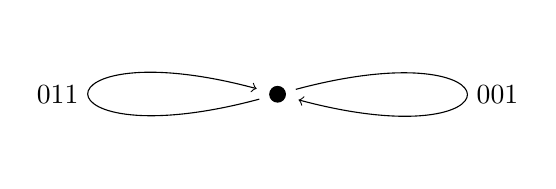
\begin{tikzpicture}[main node/.style={circle,draw,fill,inner sep=2pt,outer sep=4pt},scale=6]
    \node[main node] (1) {};
    \path
        (1) edge [loop left] node {011} (1)
            edge [loop right] node {001} (1);
\end{tikzpicture}
    \caption{Optimal code representation of the finitite state automata.}
\end{center}

\end{figure}

\section{Old idea}

A labeled finite automata generates a sequences of 0s and 1s. It is not a Markov system since the probability distribution for the next symbol is not immediately known from the current symbol. Knowing the current symbol being 0 can result in 100\% chance of generating a 1 and 100\% chance of generating a 0, depending on where in the system one is located.

\begin{figure}[ht]
    \begin{center}
    \includegraphics[width=0.5 \linewidth]{fig.png}
    \caption{The finite automata in question.}
    \end{center}
\end{figure}

We introduce names to the 5 nodes, in order from left to right: $A,B,C,D$ and $E$. The entropy per symbol is calculated using
\begin{equation}
    s = \lim_{m \rightarrow \infty} \sum_{x_1 \dots x_{m-1}} p(x_1 \dots x_{m-1})
    \sum_{x_m} p(x_m | x_1 \dots x_{m-1}) \log \frac{1}{p(x_1 \dots x_{m-1})},
\end{equation}
from the book. For convenince's sake, we can introduce a variable $z = x_1 \dots x_{m-1}$, resulting in
\begin{equation} \label{eq:z}
    s = \lim_{m \rightarrow \infty} \sum_{z} p(z)
    \sum_{x_m} p(x_m | z) \log \frac{1}{p(z)}.
\end{equation}

Next up, we need to calculate the probability of being at each node in the system. As defined by the excercise, when situated at a node with several exiting edges, one is picked at random with equal probability. Therefore, the probability of ending up at a node is proportional to the amount of edges pointing to it. For normalisation, all probabilities must of course sum to 1. This results in the following system of equations
\begin{equation}
    \begin{cases}
        p(A) = p(B) = p(D) = p(E) \\
        p(C) = 2p(A) \\
        p(A) + p(B) + p(C) + p(D) + p(E) = 1.
    \end{cases}
\end{equation}

Substituting the two upper equations into the bottom gives
\begin{equation}
    p(C) + p(C) + p(C) = 3 p(C) = 1 \iff p(C) = \frac{1}{3},
\end{equation}
which in turn gives
\begin{equation}
    p(A) = p(B) = p(D) = p(E) = \frac{1}{6}.
\end{equation}

The entropy we're looking for doesn't consider the made up nodes $A, B, C, D, E$ but the 0s and 1s which they generate. Therefore we also need to establish the probability of getting a 0 or 1 from every transition between the nodes. Most of the nodes only have one exiting edge and the last one has two exiting nodes with equal probability. Therefore
\begin{equation}
    \begin{matrix}
        p(1|A) = 1 & p(0|A) = 0 \\
        p(1|B) = 1 & p(0|B) = 0 \\
        p(1|C) = 0 & p(0|C) = 1 \\
        p(1|D) = 0 & p(0|D) = 1 \\
        p(1|E) = 1 & p(0|E) = 0
    \end{matrix}
\end{equation}
all nodes generate a desterministic symbol, even though the edge chosen is random. Therefore equation \eqref{eq:z} simplifies to
\begin{equation}
    s = \lim_{m \rightarrow \infty} \sum_z p(z) \log \frac{1}{p(z)},
\end{equation}


Is it possible to convert this to a system of 2 symbols? 011 and 001. This would turn the system into a Markov system, reducing the complexity of the calculation. The entropy would only depend on
\begin{equation}
    s = p(B) \left[ p+++ \right]
\end{equation}

\end{document}
